\chapter{Introduction}

Many quantum systems studied in condensed matter physics are experimentally
challenging to access as any interactions can destroy the carefully prepared
quantum states. As way forward, experiments with ultracold atoms in
optical lattices give us a highly contorllable environment, giving us the
opportunity to simulate and explore quantum effects and expand our current
understanding of quantum mechanics and statistical physics \cite{Gross2017}.

The central idea behind these types of experiments is to cool down neutral
atoms to micro Kelvin and below, and load them into an optical lattice. At
these temperatures atoms demonstrate quantum behaviour. The optical lattices
act as periodic potentials analogue to the periodic potential found inside
solid state crystal lattices \cite{Lewenstein2007}. Unlike to i.e. real solids
where we have limited prospects to amend a systems properties, lasers driven
by state of the art optics and electronics give us a wide range of well
controllable parameters.

\begin{figure}[h]
  \centering
  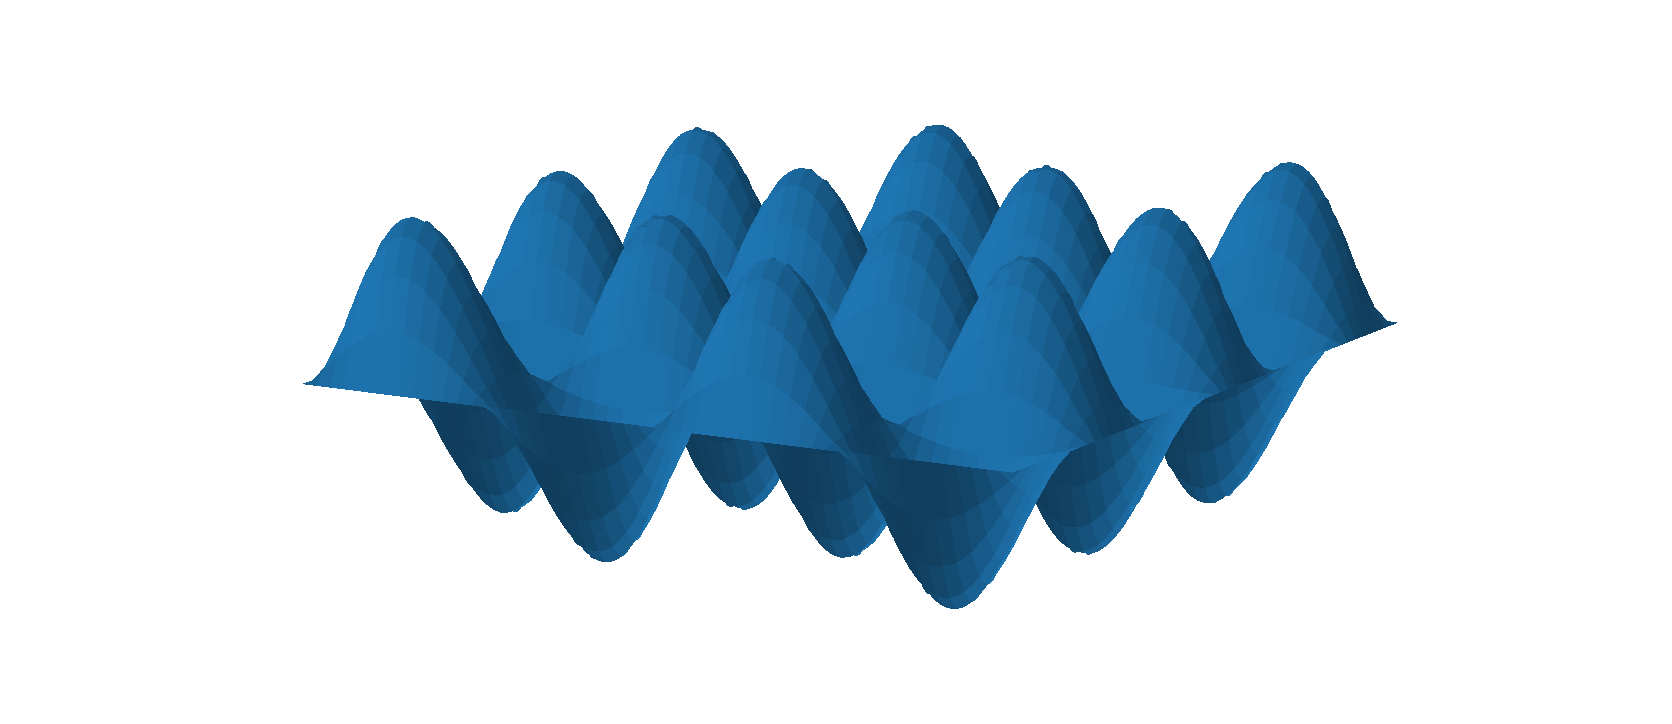
\includegraphics[width=.8\textwidth]{images/optlat/default.pdf}
  \captionsetup{width=.8\textwidth}
  \caption{Periodic potential of a 2D optical lattice. If the kinetic energy
  of the atoms is below the potential energy of the lattice, the atoms will
  locate around the potential minimas.}
  \label{fig:optlat}
\end{figure}

One of the parameters of interest is the ability to apply local potentials
to the system, that can be used to, among others, study lattice inpurities
or quantum interactions. In this work we will present and characterize one
possible implementation of such a local potential generating apparatus.

\section{Related Work}

Local manipulations of atoms inside optical lattices have been known for some
time in the embodiment of optical tweezers that allow trapping, stacking and
sorting of particles \cite{Tadmor2004}. Yet, only recently attempts to
interact with local particle clusters through high-precision time-averaged
optical potentials have been reported \cite{Roy2016}.

In the following we continue on the laid out work \cite{Hertlein2017} which
provided us with an optical setup for single-site manipulation using
\gls{aod} as well as considerations with regard to aperture limited
gaussian beam propagation.

\section{Concept}
% image of how laser beam sweepsa through single sites

% requirements:
% - order of sweep speed from physical model
% - homogeneous intensity

% dynamics

% parameters
